\chapter{Un po' di algebra lineare e la SVD}

\section{Autovalori e autovettori}
\dfn{}{
    Data una matrice $A$ di dimensione $n\times n$ se vale:
    \[
        Ax=\lambda x    
    \]
   con $\lambda \in \mathbb{R}$ e $x\in \mathbb{R}^n,\lambda$ si dice autovalore di $A$ e $x$ autovettore di $A$ associato a $\lambda$
}
Data questa definizione, e richiamando i vari concetti dell'algebra lineare, abbiamo che se vale $Av_{i} = \lambda_{i}v_{i},\forall i\in {1,\dots, n}$ allora vale anche:
\begin{align*}
    [A v_1, A v_2, \dots, A v_n] &= [\lambda_1 v_1, \lambda_2 v_2, \dots, \lambda_n v_n] \\
    \text{quindi:} \quad A[v_1, v_2, \dots, v_n] &= [v_1, v_2, \dots, v_n] \begin{pmatrix}
        \lambda_1 & 0 & \cdots & 0 \\
        0 & \lambda_2 & \cdots & 0 \\
        \vdots & \vdots & \ddots & \vdots \\
        0 & 0 & \cdots & \lambda_n
        \end{pmatrix}        
\end{align*}

Questa bellissima scrittura si può tranquillamente riassumere come: \[AV=DV\]

\subsection{Decomposizione agli autovalori}
\dfn{}{
    sia $A\in M^{n\times n}$, allora una Una decomposizione agli autovalori di $A$ è una fattorizzazione (ovvero un prodtto) di questo tipo:
    \[
      A=VDV^{-1}
    \]
    Dove $V=[v_1, v_2, \dots, v_n]$ è la matrice con colonne gli autovettori $v_1$ di $A$ e $D$ è una matrice diagonale che ha sulla diagonale gli autovalori di $A$ associati alle colonne di $V$
}
Se $A$ ha una decomposizione agli autovalori
allora si dice che $A$ è \textbf{diagonalizzabile}; in
caso contrario $A$ si dice \textbf{non
diagonalizzabile} (o defettiva). \\

Se $A$ ha $n$ autivalori distinti, allora $A$ è diagonalizzabile

\section{Vettori ortogonali e ortonormali}
\dfn{}{
    Siano $v_1, v_2, \dots, v_m$ vettori di $R^n$, si dicono \textbf{ortognonali} se:
    \[
        v_i^T v_j = 0, \quad \text{se } i \neq j
    \]
    Si può scrivere anche:
    \[
        \langle  v_i, v_j \rangle = 0, \quad \text{se } i \neq j
    \]
    Ovvero il prodotto scalare
}
Questa relazione di vettori si collega molto bene con i vettori ortonormali:
\dfn{}{
    Siano $v_1, v_2, \dots, v_m$ vettori di $R^n$, si dicono \textbf{ortonormali} se sono ortogonali w di lunghezza unitaria, ovvero $v_i^T v_j = \|v_i\|= \delta_{ij}$
    dove
    \[
        \delta_{ij} = 
            \begin{cases}
                1 \quad \text{se } i=j \\
                0 \quad \text{se } i\neq j
            \end{cases}
    \]
}
\subsection{Matrici ortogonali}
\dfn{}{
    Una matrice $W$ di dimensione $n \times n$ si dice ortogonale se le sue colonne sono vettori ortonormali
}
Un esempio semplice:
\esempio{
  \[
    W = \begin{pmatrix}
        \frac{1}{\sqrt{3}} & 0 & \frac{1}{\sqrt{2}} \\
        \frac{1}{\sqrt{3}} & 1 & \frac{1}{\sqrt{2}} \\
        \frac{1}{\sqrt{3}} & 0 & 0
        \end{pmatrix}
  \]
}
le matrici ortogonali hanno diverse proprietà:
\begin{enumerate}
    \item $W^T = W^{-1}$
    \item $\forall x \in R^n, \|x\|_2=\|W x\|_2$
\end{enumerate}


\section{SVD}
\nt{
  Fonti: 
  \begin{itemize}
      \item \href{https://www.youtube.com/watch?v=vSczTbgc8Rc}{Visualizzazione geometrica}
      \item \href{https://www.youtube.com/watch?v=vSczTbgc8Rc}{Visualizzazione vettori ortogonali e dimostrazione minimo quadrato}
      \item \href{https://gregorygundersen.com/blog/2018/12/20/svd-proof}{Dimostrazione SVD}
  \end{itemize}
}
Prima di iniziare ad introdurre metodi di approssimazione, e' necessario esplorare uno dei teoremi finali dell'algebra lineare: la \textbf{SVD} (Singular Value Decomposition). Questo teorema sara' fondamentale per descrivere vari modelli di ottimizzazione e approssimazione per motivi che vedremo dopo.\\
\\
\subsection{Introduzione}
Un modo per arrivare alla SVD e' porci la seguente domanda: data una matrice $ A \in M(\mathbb{R})_{n \times m} $, esistono $ m $ vettori ortonormali in $ \mathbb{R}^m $ la cui immagine e' sempre un insieme di $ m $ vettori ortogonali (se $ m > n $ allora $ m -n $ vettori dell'immagine saranno nulli) in $ \mathbb{R}^n $? Proviamo a scrivere la domanda in modo piu' matematico:
\[
  \exists V \in M(\mathbb{R})_{m}, U \in M(\mathbb{R})_n, \Sigma \in M(\mathbb{R})_{n \times m}. V, U \text{ ortonormali, } \Sigma \text{ diagonale (rettangolare)}. \forall A \in M(\mathbb{R})_{n \times m}:
\]
\[
 AV = U\Sigma
\]
dove $ V $ ha come colonne i vettori ortonormali del dominio, $ U $ ha come colonne vettori ortonormali (se $ n > m $ le ultime $ n-m $ colonne non importano e possono essere nulle) che moltiplicate per i corrispondenti scalari sulla diagonale della matrice $ \Sigma $ formano l'immagine ortogonale di $ V $. Dato che $ V $ e' ortonormale, posso riscrivere l'equazione come scomposizione di $ A $:
\[
A = U\Sigma V^T
\]
Questa e' la scomposizione di cui la SVD ci assicura l'esistenza per qualsiasi matrice $ A $, formalmente:
\thm{Singular Value Decomposition}{
  Per qualsiasi $ A \in M(\mathbb{R})_{n \times m} $, esistono:
  \begin{itemize}
    \item $ U $ ortonormale $ n \times n $
    \item $ V $ ortonormale $ m \times m $
    \item $ \Sigma $ rettangolare diagonale $ n \times m $
  \end{itemize}
  Tali che:
  \[
    A = U\Sigma V^T
  \]
}
\mlenma{Lemma 1}{
  Per una qualsiasi matrice $ A \in M(\mathbb{R})_{n \times m} $, si ha che:
  \begin{itemize}
    \item $ A^T A \in M(\mathbb{R})_n $ semidefinita positiva
    \item $ A A^T \in (\mathbb{R})_m $ semidefinita positiva
  \end{itemize}
}
\pf{}{
  Dimostra (forse)
}

\pf{Dimostrazione SVD}{
  Sia $ A \in M(\mathbb{R})_{n \times m} $. Per Lemma 1, sappiamo che $ A^T A $ e' una matrice semidefinita positiva, quindi, per il teorema spettrale, puo' essere scomposta come:
  \[
  A^T A = V \Lambda V^T
  \]
  dove $ V \in M(\mathbb{R})_m $ e' una matrice ortonormale e $ \Lambda \in M(\mathbb{R})_m $ e' la matrice diagonale di autovettori ordinati $ \lambda_1 \geq ... \geq \lambda_m $ tali che $ Av_1 = \lambda_1 v_1 $. Definiamo ora $ n $ vettori $ u_i $ nel seguente modo, dove $ \sigma_i = \sqrt{\lambda_i} $:
  \[
  u_i = \begin{cases}
  \frac{Av_i}{\sigma_i} & \lambda_i \neq 0 \\
  \underline{0} & \lambda_i = 0
  \end{cases} 
  \]
  Dato che $ A^T A $ ha lo stesso rango di $ A $ (dim. nella fonte), se $ A $ ha rango massimo allora $ \forall i. \sigma_i > 0 $ (perche' si puo' dimostrare che $ A^T A $ diventa \textbf{definita} positiva); se $ r = rank(A) < min(n, m) $, allora gli ultimi $ min(n, m) - r $ valori singolari saranno nulli. (Da riguardare perche non sono sicurissimo)
  Si puo' dimostrare che $ u_i $ sono autovettori di $ A A^T $:
  \begin{align*}
    A A^T u_i &= A A^T \frac{Av_i}{\sigma_i} \\
    &= A \frac{\sigma_i^2 v_i}{\sigma_i} \\
    &= \sigma^2\frac{A v_i}{\sigma_i} \\
    &= \sigma^2 u_i
  \end{align*}
  E che sono unitari:
  \begin{align*}
    u_i^T u_i &= \frac{v_i^T A^T}{\sigma_i} \frac{Av_i}{\sigma_i} \\
    &= \frac{v_i^T \sigma^2 v_i}{\sigma^2} \\
    &= v_i^T v_i = 1
  \end{align*}

  Essendo autovettori unitari di una matrice semidefinita positiva ($ A A^T $), la matrice $ U \in M(\mathbb{R})_n $ che ha come colonne $ u_i $ e' ortonormale. Usando le matrici possiamo scrivere:
  \[
   Av_i = \sigma_i u_i \implies AV = U \Sigma 
  \]
  dove $ \Sigma \in M(\mathbb{R})_{n \times m} $ ha sulla diagonale $ min(n, m) $ valori singolari ($ \sigma_1,...,\sigma_{min(n, m)} $) e il resto e' 0.
  \[
  A = U \Sigma V^T
  \]
}

\subsection{Interpretazione geometrica}
Questa scomposizione puo' essere interpretata in modo geometrico. Immaginiamo di moltiplicare un vettore $ x $ per la scomposizione di $ A $:
\begin{itemize}
  \item La matrice $ V^T $, essendo ortonormale, applica una rotazione a $ x $ senza variarne il modulo. Essendo trasposta, che per le matrici ortonormali corrisponde con l'inversa, al posto di spostare i vettori base ai vettori di $ V $ fa il contrario.
  \item La matrice $ \Sigma $ puo' essere scomposta in due parti:
    \begin{itemize}
      \item La matrice $ m \times m $ diagonale, che ha come valori diagonali gli $ m $ valori singolari. Dato che e' diagonale, applica solo un'allungamento/restrizione di x ruotato.
      \item Una matrice $ n \times m $ rettangolare diagonale con solo valore $ 1 $. Serve per portare il vettore nel nuovo spazio vettoriale. 
      \begin{center}
        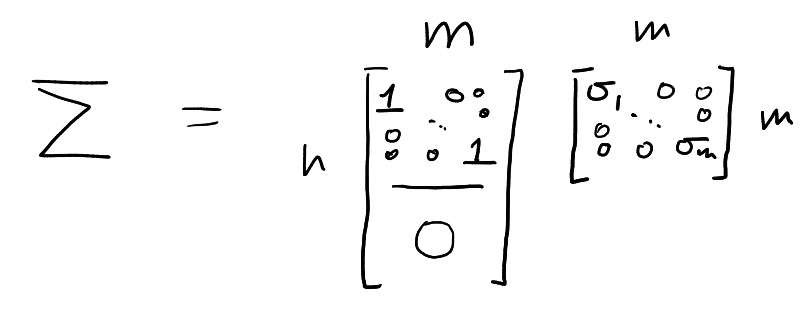
\includegraphics[width=0.5\textwidth]{img/2024-11-20-17-27-02.png}
      \end{center}
    \end{itemize}
  \item Infine la matrice $ U $ ortonormale ruota il vettore nello spazio del codominio $ \mathbb{R}^n $, spostando la base sui vettori di $ U $.
\end{itemize}

\ex{Mappa da sfere a elissoidi}{
  Consideriamo una cironferenza unitaria in $ \mathbb{R}^2 $:
\begin{center}
  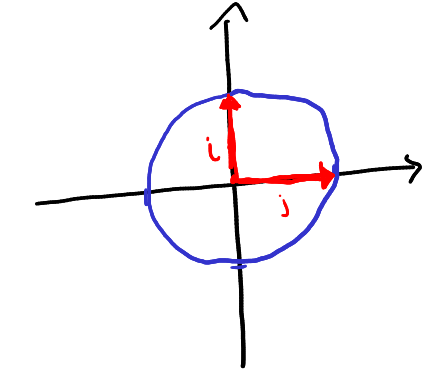
\includegraphics[width=0.3\textwidth]{img/2024-11-21-09-53-22.png}
\end{center}
Applichiamo la trasformazione lineare definita dalla matrice $ A \in M(\mathbb{R})_{3 \times 2} $. Come abbiamo visto, qualunque matrice puo' essere scomposta come due matrici di rotazione e una di "allungamento". Vediamo i vari passaggi:
\begin{itemize}
  \item Applicando la prima rotazione, la nostra figura non cambia dato che e' una circonferenza:

\begin{center}
  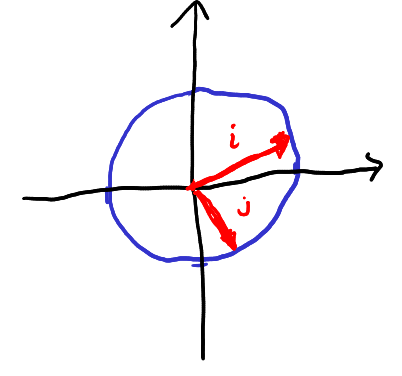
\includegraphics[width=0.3\textwidth]{img/2024-11-21-10-02-10.png}
\end{center}
  \item Moltiplicando per la matrice diagonale, la circonferenza viene allungata lungo due assi principali (i vettori della base canonica che sono stati roteati da $ V^T $). Abbiamo quindi un'ellisse:

\begin{center}
  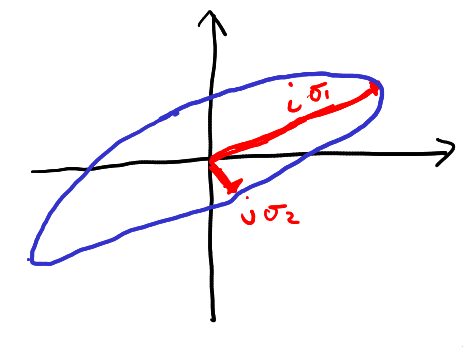
\includegraphics[width=0.3\textwidth]{img/2024-11-21-10-02-40.png}
\end{center}
  \item Spostiamo l'ellisse in $ \mathbb{R}^3 $:

\begin{center}
  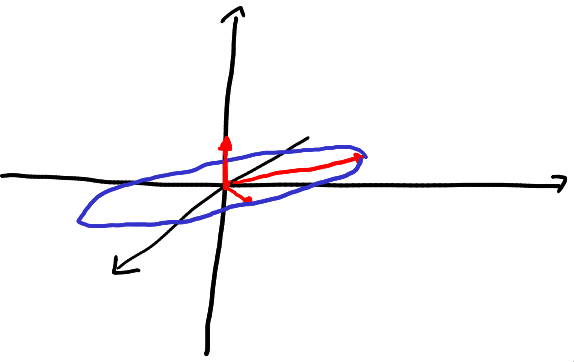
\includegraphics[width=0.3\textwidth]{img/2024-11-21-10-03-11.png}
\end{center}
  \item Manca solo l'ultima rotazione applicata da $ U $, questa volta in $ 3 $ dimensioni:

\begin{center}
  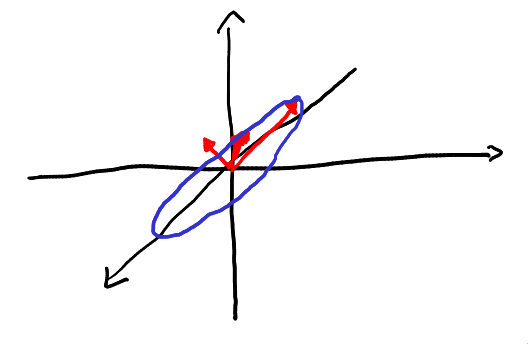
\includegraphics[width=0.3\textwidth]{img/2024-11-21-10-03-38.png}
\end{center}
  
\end{itemize}
  Per questo motivo, possiamo dire che le matrici $ n \times m $ trasformano sfere in $ \mathbb{R}^m $ in elissoidi a $ n $ dimensioni.
}

Quindi i \textbf{valori singolari} $ \sigma_1,...,\sigma_{min(n, m)} $ sono i coefficenti scalari che moltiplicano i vettori lungo $ min(n, m) $ assi ortogonali. 

\subsection{Applicazioni}
La SVD e' uno strumento utilizzato moltissimo per problemi di ottimizzazione e di aprossimazione, in quanto e' applicabile universalmente e fornisce informazioni molto importanti per l'analisi dei dati. La lista ordinata in modo discendente rispetto a quanto la matrice "allunga" i vettori lungo una certa direzione (vettori singolari destri e sinistri ???) e' utilizzata per la PCA (Principal Component Analisis ???) e per l'aprossimazione di matrici. Inoltre, la SVD e' utilizzata per risolvere il problema dei minimi (o massimi) quadrati, come vedremo prossimamente.

\section{Fattorizzazione in Valori Singolar (SVD)}
La fattorizzazione in valori singolari non è altro che uno strumento che permette di rappresentare una matrice $A\in M^{m\times n}$ attraverso una matrice diagonale. Vediamo come:
\teorema{
    Sia $A\in M^{m\times n}$ una matrice di rango $k$ con $k\leq n\leq m$. Allora esistono:
    \begin{itemize}
        \item una matrice ortognonale $U\in M^{m\times m}$
        \item una matrice ortogonale $V\in M^{n\times n}$
        \item una matrice diagonale $\Sigma \in M^{m\times n}$
    \end{itemize}
    tali che:
    \[
        A=U\Sigma V^T, \quad \Sigma = 
        \begin{pmatrix}
            \sigma_1 & 0 & \cdots & 0 \\
            0 & \sigma_2 & \cdots & 0 \\
            \vdots & \vdots & \ddots & \vdots \\
            0 & 0 & \cdots & \sigma_n \\
            \vdots & \vdots &  & \vdots & \\
            0&0&\cdots&0
        \end{pmatrix}
    \]
}
\begin{itemize}
    \item Gli elementi $\sigma_1\geq\sigma_2\geq\dots\sigma_n\geq 0$ sono i cosidetti  \textbf{valori singolari di $A$}
    \item Mentre il rango $k$ è uguale al numero di valori singolari positivi, cioè $k=rango(A)\iff (\sigma_1\geq\sigma_2\geq\dots\sigma_k > 0\land \sigma_{k+1}=\dots = \sigma_n = 0)$
    \item Le colonne si $U=(u_1,u_2,\dots, u_m)$ e di $V=(v_1,v_2,\dots,v_n)$ sono, rispettivamente, i \textbf{vettori singolari sinistri e destri di $A$} associati ai valori singolari $\sigma_i$ e formano una base ortonormale di $R^m$ e $R^n$ , rispettivamente, poichè vale la relazione:
    \[
            Au_i = \sigma_i v_i
    \]
\end{itemize}


Questo teorema porta a un'implicazione piuttosto interessante, inffatti si ha: 

\[
    A^T A = (U\Sigma V^T)^T (U\Sigma V^T) = V\Sigma^T U^T U\Sigma V^T
\]
dato che $U$ è ortogonale si "annulla" con la sua trasposta, quindi continua con 
\[
    V\Sigma^T \Sigma V^T = V 
    \begin{pmatrix}
        \sigma_1^2 & 0 & \cdots & 0 \\
        0 & \sigma_2^2 & \cdots & 0 \\
        \vdots & \vdots & \ddots & \vdots \\
        0 & 0 & \cdots & \sigma_n^2 \\
    \end{pmatrix} V^T
\]

Inoltre:
\[
    \sigma_i =\sqrt{\lambda_i}, i=\dots,n 
\]
Dove $\lambda_i$ non è che l'autovalore di $A^TA$, si ha quindi:
\begin{itemize}
    \item $\sigma_1 =\sqrt{\lambda_{max}}=\sqrt{\rho}=\|A\|$
    \item $\sigma_k =\sqrt{\lambda_{min}} \Rightarrow \|A^{-1}\| = \frac{1}{\sigma_k}$
\end{itemize}

\subsubsection{numero di condizione}

\dfn{Numero di condizione}{
    Si dice \textbf{numero di condizione di $A$} tale valore:
    \[
        K_2(A)=\frac{\sigma_1}{\sigma_k}    
    \]
    Dove $\sigma_k$ è il valore singolare minimo di $A$ e $k$ è il rango della matrice, quindi $k\leq \min(m,n)$ \\
    Un'altra definizione di questo valore è:
    \[
        K_2(A) = \|A\|\cdot \|A^{-1}\|
    \]
}
Un \red{numero di condizionamento basso} (vicino a 1) indica che la matrice è ben condizionata. \red{Ciò significa che piccole variazioni negli input producono piccole variazioni negli output}, viceversa \red{un numero di condizionamento alto} indica che la matrice è mal condizionata. Ciò \red{significa che piccole variazioni negli input possono causare grandi variazioni negli output}
